\documentclass[border=10pt]{standalone}

\usepackage{tikz}
\usepackage{tikzsymbols}
\usetikzlibrary{calc,patterns,shapes.geometric}

\def\centerarc[#1](#2)(#3:#4:#5){\draw[#1] ($(#2)+({#5*cos(#3)},{#5*sin(#3)})$) arc (#3:#4:#5);}

\begin{document}
	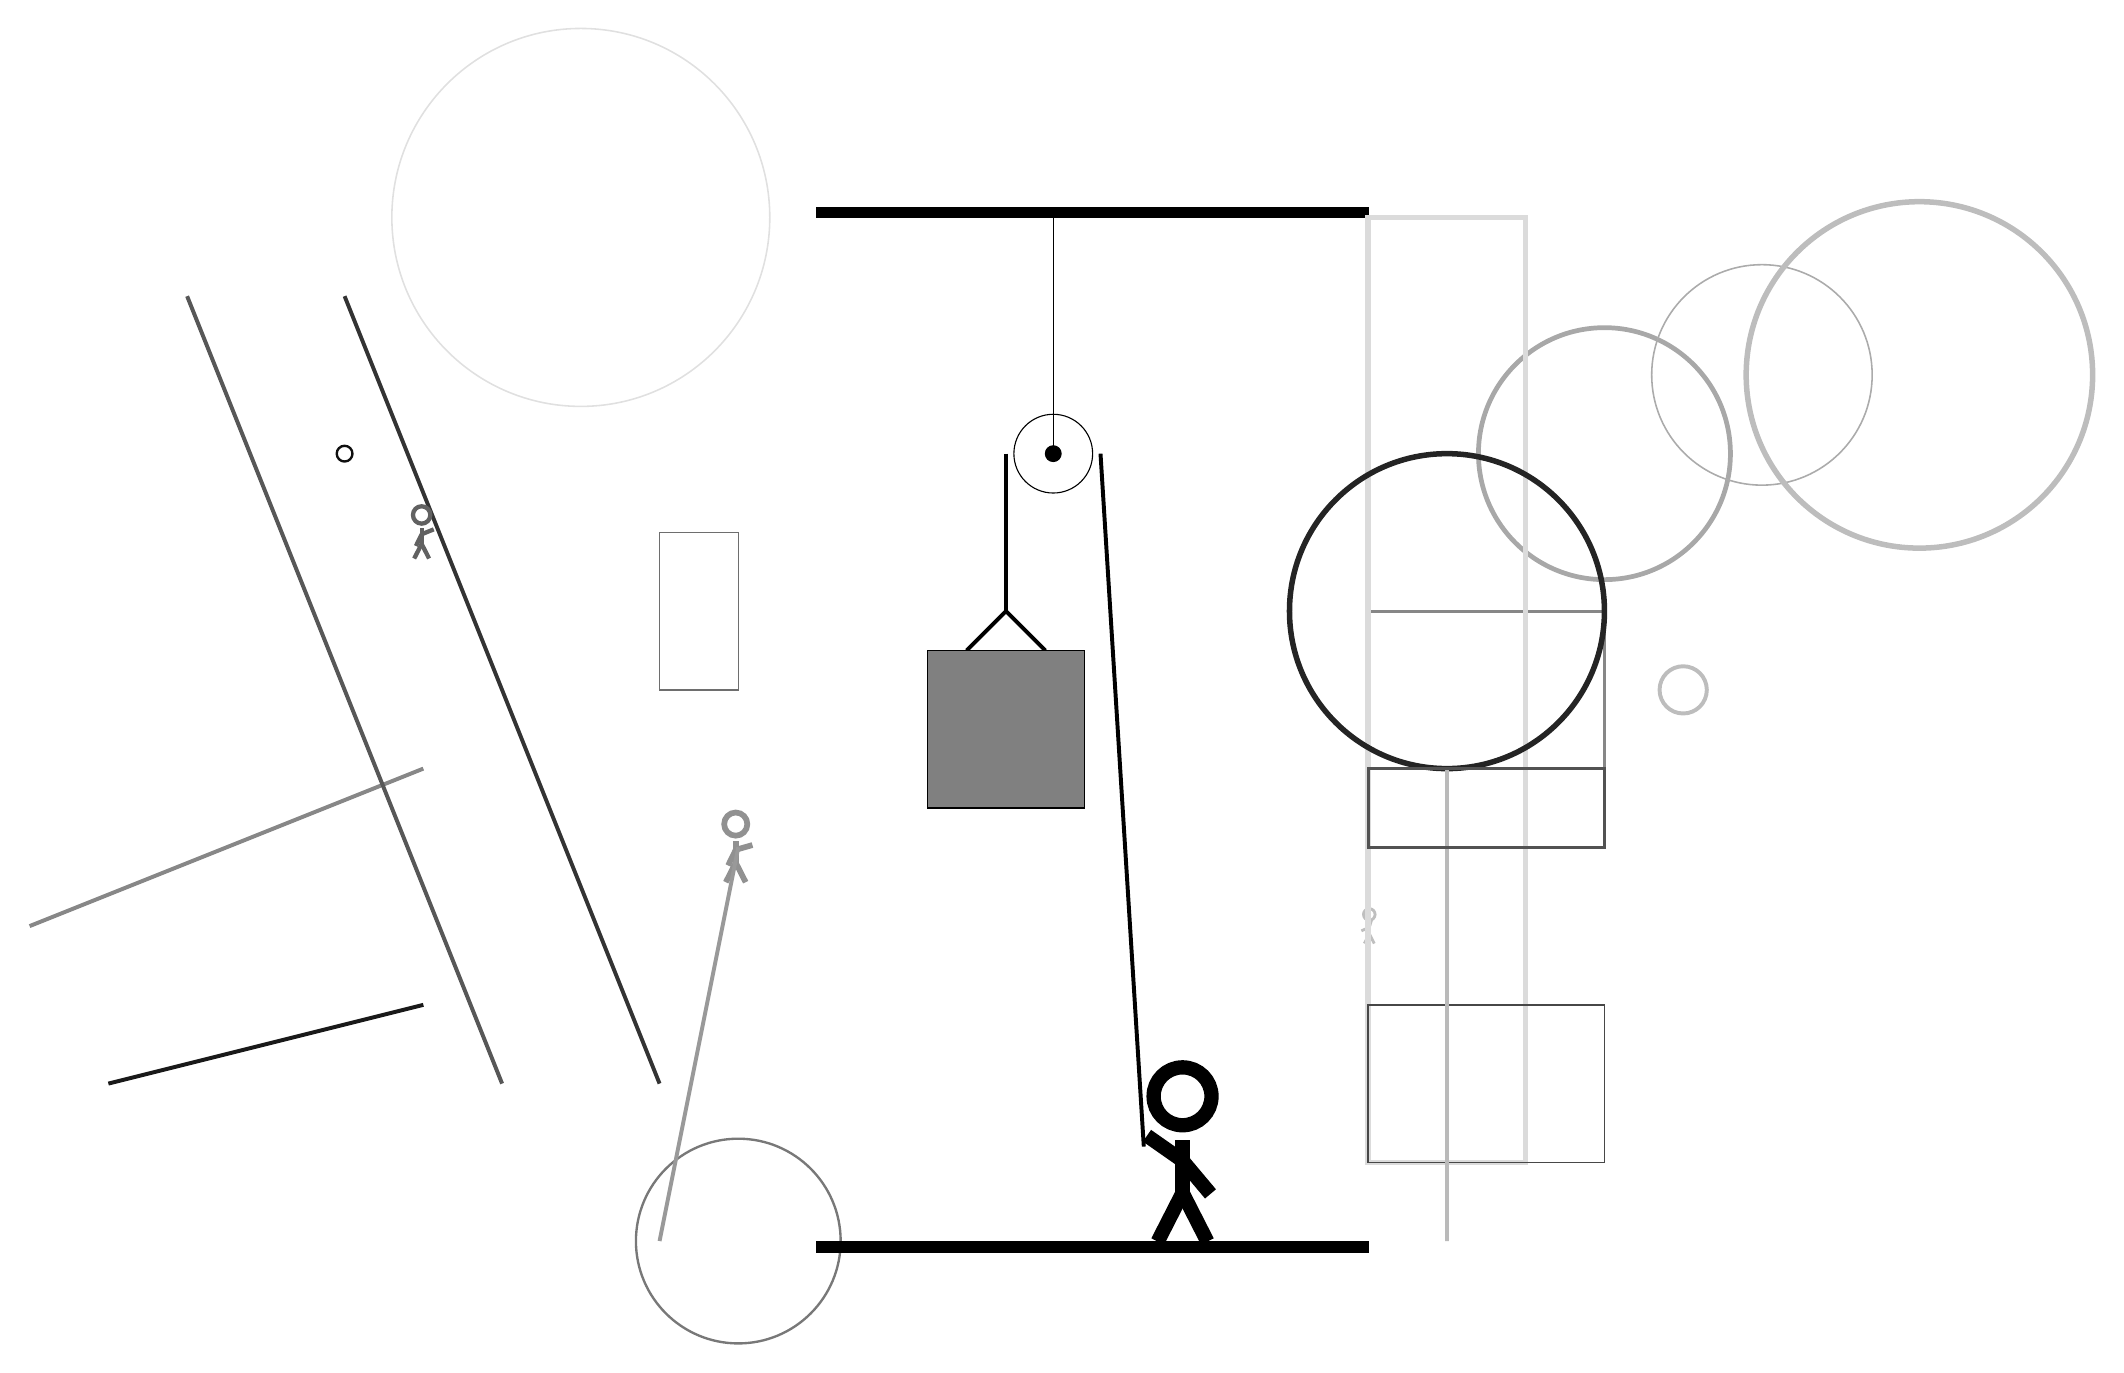
\begin{tikzpicture}
		%%%%% START %%%%%
		
		\draw[fill=black] (-2, 10) rectangle (5, 10.125);
		
		\draw (1, 7) circle (0.5);
		\draw[fill=black] (1, 7) circle (0.1);
		\draw (1, 10) -- (1, 7);
		
		\draw[line width=0.5mm] (-0.1, 4.5) -- (0.4, 5.0) -- (0.9, 4.5);
		\draw[fill=black!50] (-0.6, 4.5) rectangle (1.4, 2.5);
		
		\draw[line width=0.5mm] (0.4, 7) -- (0.4, 5.0);
		\centerarc[line width=0.5mm](1, 7)(0:180:0.6);
		\draw[line width=0.5mm](1.6, 7) -- (2.15, -1.8);
		
		\draw [line width=0.6mm, color=black!34](8, 7) circle (1.6);
		
		\draw [line width=0.3mm, color=black!53](-3, -3) circle (1.3);
		\draw [line width=0.2mm, color=black!12](-5, 10) circle (2.4);
		\node[line width=0.3mm, color=black!25] at (5, 1) {\Strichmaxerl[2][24][73]};
		
		\draw[line width=0.5mm, color=black!90](-7, 0) -- (-11, -1);
		\draw[line width=0.4mm, color=black!20] (5, 3) rectangle (8, 3);
		\draw[line width=0.4mm, color=black!47] (5, 5) rectangle (8, 3);
		\node[line width=0.6mm, color=black!43] at (-3, 2) {\Strichmaxerl[4][64][16]};
		\draw[line width=0.7mm, color=black!14] (5, 10) rectangle (7, -2);
		\draw[line width=0.2mm, color=black!72] (5, -2) rectangle (8, 0);
		\draw[line width=0.2mm, color=black!57] (-4, 4) rectangle (-3, 6);
		\draw [line width=0.7mm, color=black!86](6, 5) circle (2.0);
		\draw[line width=0.5mm, color=black!80](-4, -1) -- (-8, 9);
		
		\draw [line width=0.3mm, color=black!94](-8, 7) circle (0.1);
		\draw[line width=0.5mm, color=black!40](-3, 2) -- (-4, -3);
		\draw[line width=0.4mm, color=black!27] (6, -3) rectangle (6, 3);
		\draw [line width=0.2mm, color=black!33](10, 8) circle (1.4);
		
		\draw [line width=0.7mm, color=black!26](12, 8) circle (2.2);
		\draw[line width=0.5mm, color=black!47](-7, 3) -- (-12, 1);
		\node[line width=0.6mm, color=black!62] at (-7, 6) {\Strichmaxerl[3][64][22]};
		\draw[line width=0.5mm, color=black!66](-6, -1) -- (-10, 9);
		\draw [line width=0.5mm, color=black!26](9, 4) circle (0.3);
		
		\draw[line width=0.4mm, color=black!68] (5, 2) rectangle (8, 3);
		
		\node at (2.6, -1.9) {\Strichmaxerl[10][-35][-50]};
		
		\draw[fill=black] (-2, -3) rectangle (5, -3.15);
		
		%%%%% END %%%%%
	\end{tikzpicture}
\end{document}